\section{多边形与圆}

\subsection{多边形的面积}
\begin{frame}
\pause
三角形的面积可以用叉积快速求，多边形的面积可以以某个点为中心，把多边形分成若干个三角形，然后对所有三角形面积求和相加。

\pause
同时，叉积计算的是有向面积，所以中心也可以在多边形之外。

\pause
一般我们选取中心为原点$(0,0)$，这样可以避免向量减法，减小常数。
\end{frame}

\subsection{点在多边形内的判定}
\begin{frame}
\pause
点在多边形内的判定一般用射线法。

\pause
从询问点随机一个角度射出一条射线，如果射线与奇数条多边形的边相交则在多边形内，否则不在。

\pause
需要注意的是如果射线正好设在了某两条线段的交点上则不方便处理，重新随机一条射线就可以了。
\end{frame}

\subsection{圆和直线的交点}
\begin{frame}
\frametitle{求圆$(x,y,R)$和直线$AB$的交点}

\pause
方法一：直接解方程求出交点坐标。

\pause
方法二：首先求出圆心到直线的距离dis。如果$dis>R$则显然无交点。

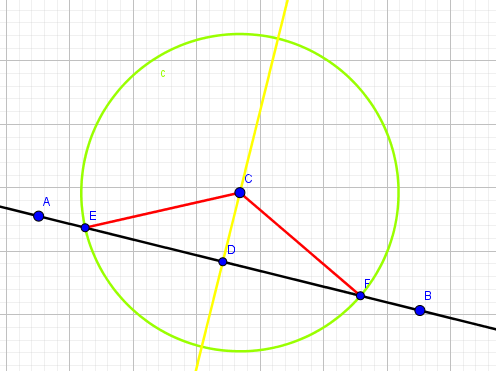
\includegraphics[width=4cm]{geometry/circle.png}

作出C到AB的垂足D。那么$\angle ECD=\angle FCD=acos(dis/R)$。

这样我们就可以得到CE和CF的极角。然后就可以计算出E和F的坐标。
\end{frame}

\subsection{圆和圆的交点}
\begin{frame}
\frametitle{求圆$(x_1,y_1,R_1)$和圆$(x_2,y_2,R_2)$的交点}

\pause
方法一：最直接的方法：解方程。

\pause
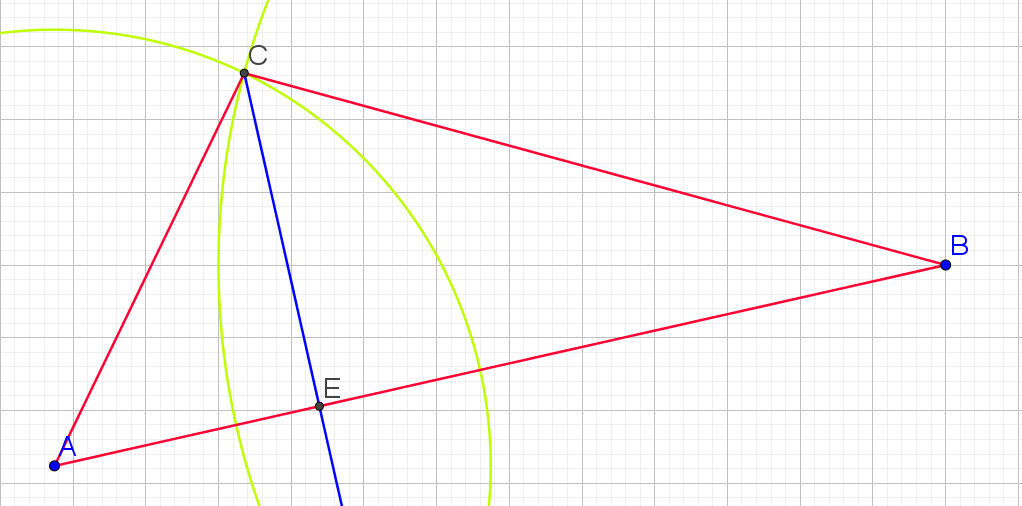
\includegraphics[width=6cm]{geometry/circle2.png}

方法二：我们已知$|AC|=R_A,|BC|=R_B,|AB|$，可以用海伦公式求出$\Delta ABC$的面积，然后得到$CE$

这样也可以知道$|AE|$，就能求出E的坐标，然后再求出点C

\pause
方法三：现在知道了$\overrightarrow{AB}$的极角，可以用余弦定理求出$\angle CAB$，那么就知道了$\overrightarrow{AC}$的极角，直接得到C的坐标。

一般采用方法三，方法二要特判E在线段AB的延长线上的情况。
\end{frame}

\subsection{点和圆的切线}
\begin{frame}
\frametitle{求点B到圆A的切线}
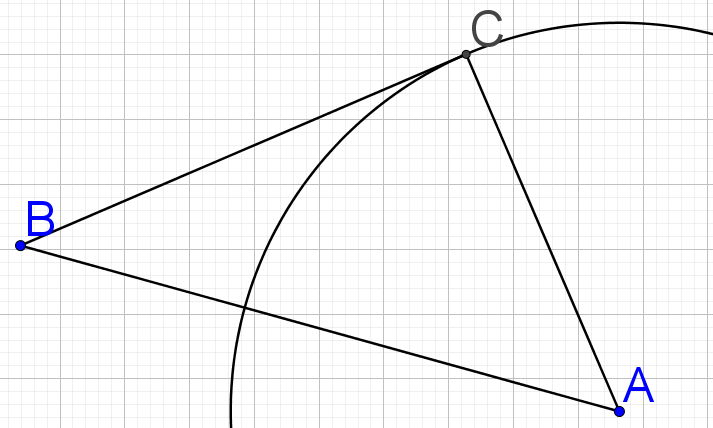
\includegraphics[height=5cm]{geometry/circle3.png}

\pause
利用反三角函数求出$\angle CBA$，然后得到$\overrightarrow{BC}$的极角，从而得到C的坐标
\end{frame}

\subsection{圆与圆公切线}
\begin{frame}
\frametitle{求圆A和圆B的公切线}
\pause
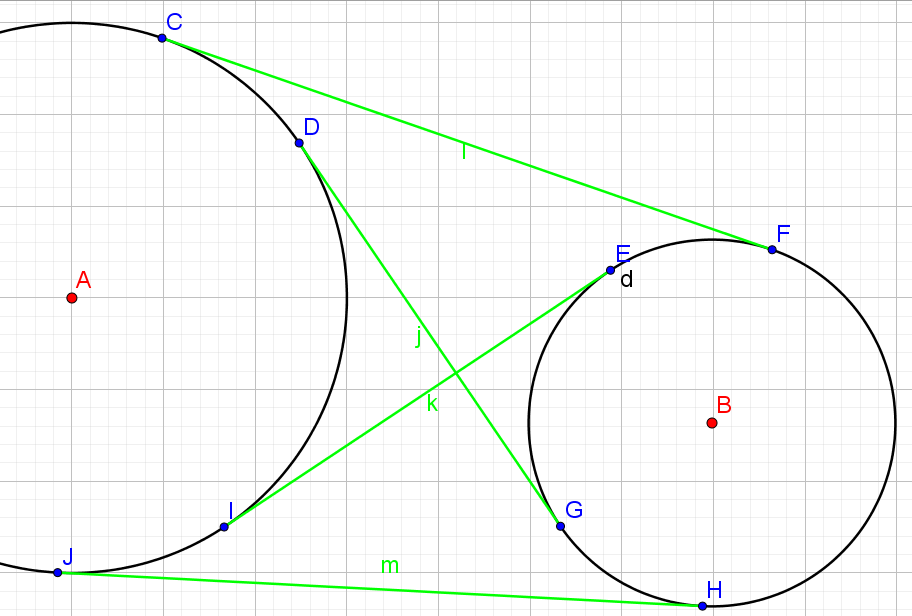
\includegraphics[height=5cm]{geometry/circle4.png}

圆与圆有4条公切线，分别为两条内公切线和两条外公切线
\end{frame}

\begin{frame}
\frametitle{求圆A和圆B的公切线}
\framesubtitle{Case1:内公切线}
\pause
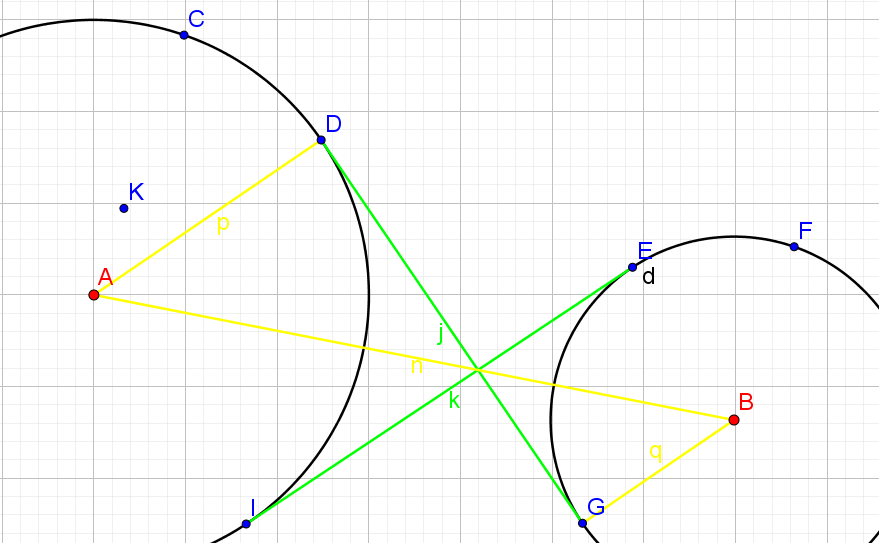
\includegraphics[height=4cm]{geometry/circle5.png}

可以先求出$\angle DAB$，然后求出点D
\begin{displaymath}
    \angle DAB=acos\left( \frac{R_A}{ |AB| * \frac{R_A}{R_A+R_B} } \right)=acos\left( \frac{R_A+R_B}{|AB|} \right)
\end{displaymath}
\end{frame}

\begin{frame}
\frametitle{求圆A和圆B的公切线}
\framesubtitle{Case2:外公切线}
\pause
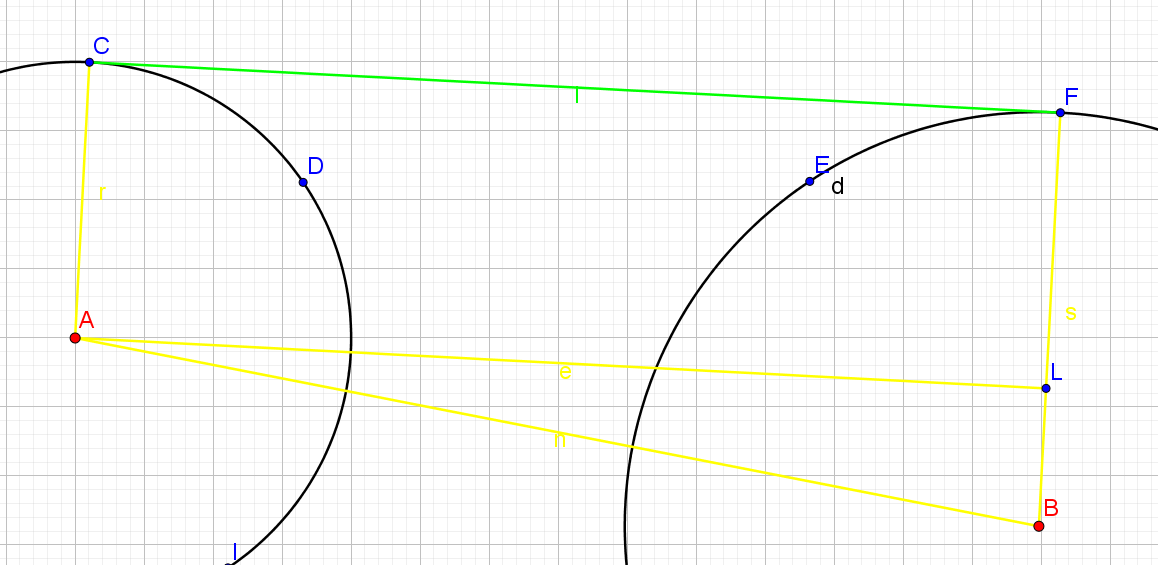
\includegraphics[height=4cm]{geometry/circle6.png}

可以先求出$\angle CAB$，然后求出点C
\begin{displaymath}
    \angle CAB=asin\left( \frac{R_B-R_A}{|AB|} \right)+\frac{\pi}{2}
\end{displaymath}
同时注意到sin是可以为负数的，所以也可以处理$R_B<R_A$的情况
\end{frame}
